\begin{figure}[H]
    \centering
    \foreach \l in {0,...,10}
    {
      \includegraphics[width=4.2cm]{linewidth/pattern\l-45.png}%
    }%
    \caption{
      Line Mode with Pulse Width at Maximum. These pleasing patterns were created by moving the cursor around a bit during painting.
      }
\end{figure}
\clearpage
\section*{line mode} 
\label{sec:linemode}
\lstset{style=6502Style}

\begin{definition}[Jeffrey Says\index{Jeffrey Says}]
\setlength{\intextsep}{0pt}%
\setlength{\columnsep}{3pt}%
\begin{wrapfigure}{l}{0.12\textwidth}

\includegraphics[width=\linewidth]{src/callout/psych.png} 
\end{wrapfigure}
\textbf{Press L to turn on and off} the Line Mode - a bit like drawing with the Aurora Borealis.\\
\textbf{Press W to adjust line width:} Sets the width of the lines produced in Line Mode.
\\
\\
\end{definition}
'Line Mode' is a completely different mode of painting. It involves no use of patterns at all. In fact it
is so completely true to its name that it consists simply of a line of vertical pixels that shoot down
the screen from underneath the cursor. The length of the line is determined by 'Line Width', with a maximum
'width' of 7 pixels high and a minimum of 1 pixel high.
\begin{figure}[H]
    \centering
    \foreach \l in {0,...,6}
    {
      \includegraphics[width=1.2cm]{linemode/pattern1-\l-45.png}%
      \hspace{0.2cm}
    }%
    \caption{
      Line Mode, a line of pixels that shoot down the screen, shown at the 7 different possible settings of 'Line Width'
      Here shown with 'X-Symmetry' so that there are two lines instead of one.
      }
\end{figure}
Since it is a completely free-standing painting mode it makes no use of the painting algorithm that has dominated
our discussion of Psychedelia until now. Let's take a look at how it worked.

\clearpage
\textbf{Lines 1275-1294. \icode{\textbf{JustLPressed\index{JustLPressed}}}} 
\begin{lstlisting}[caption=From \icode{CheckKeyboardInput\index{CheckKeyboardInput}}.,escapechar=\%]
JustLPressed%\index{JustLPressed}%   
        ; 'L' pressed. Turn line mode on or off.
        LDA lineModeActivated%\index{lineModeActivated}%
        EOR #$01
        STA lineModeActivated%\index{lineModeActivated}%
        ASL 
        ASL 
        ASL 
        ASL 
        TAY 

        ; Briefly display the new linemode on the bottom of the screen.
        JSR ClearLastLineOfScreen%\index{ClearLastLineOfScreen}%
        LDX #$00
_Loop   LDA lineModeSettingDescriptions,Y
        STA lastLineBufferPtr,X
        INY 
        INX 
        CPX #$10
        BNE _Loop
        JMP WriteLastLineBufferToScreen%\index{WriteLastLineBufferToScreen}%
        ; Returns
\end{lstlisting}

\clearpage

\textbf{Lines 1275-1294. \icode{\textbf{JustLPressed\index{JustLPressed}}}:} 
Pressing \icode{L} toggles line mode on or off. Line mode's on/off state is 
stored in \icode{lineModeActivated\index{lineModeActivated}}, with \icode{\$00} meaning 'off' and
\icode{\$01} meaning 'on'. This means we can use a neat, economical trick
for toggling the value every time the user presses the 'L' key:

\begin{lstlisting}[escapechar=\%]
        LDA lineModeActivated%\index{lineModeActivated}%
        EOR #$01
        STA lineModeActivated%\index{lineModeActivated}%
\end{lstlisting}

The \icode{EOR} statement performs an exclusive-or that has the neat property of
turning \icode{\$00} into \icode{\$01} and \icode{\$01} into \icode{\$00} - equivelent
to switching a value on or off.

This is what the the bit by bit operation looks like when '\icode{EOR \$01}' turns
\icode{trackingActivated\index{trackingActivated}} 'on':

\begin{figure}[H]
  {
    \setlength{\tabcolsep}{3.0pt}
    \setlength\cmidrulewidth{\heavyrulewidth} % Make cmidrule = 
    \begin{adjustbox}{width=7cm,center}

      \begin{tabular}{rllllllll}
        \toprule
        Byte & Bit 7 & Bit 6 & Bit 5 & Bit 4 & Bit 3 & Bit 2 & Bit 1 & Bit 0        \\
        \midrule
        \$00 & 0 & 0 & 0 & 0 & 0 & 0 & 0 & 0 \\
        \$01 & 0 & 0 & 0 & 0 & 0 & 0 & 0 & 1 \\
        \midrule
        Result & 0 & 0 & 0 & 0 & 0 & 0 & 0 & 1 \\
        \addlinespace
        \bottomrule
      \end{tabular}

    \end{adjustbox}

  }\caption*{X-OR'ing \$01 and \$00 gives \$01, the 'on' value for \icode{lineModeActivated\index{lineModeActivated}}.}
\end{figure}

And this is what it looks like when \icode{EOR \$01} turns \icode{lineModeActivated\index{lineModeActivated}} 'off' again:
\begin{figure}[H]
  {
    \setlength{\tabcolsep}{3.0pt}
    \setlength\cmidrulewidth{\heavyrulewidth} % Make cmidrule = 
    \begin{adjustbox}{width=7cm,center}

      \begin{tabular}{rllllllll}
        \toprule
        Byte & Bit 7 & Bit 6 & Bit 5 & Bit 4 & Bit 3 & Bit 2 & Bit 1 & Bit 0        \\
        \midrule
        \$01 & 0 & 0 & 0 & 0 & 0 & 0 & 0 & 1 \\
        \$01 & 0 & 0 & 0 & 0 & 0 & 0 & 0 & 1 \\
        \midrule
        Result & 0 & 0 & 0 & 0 & 0 & 0 & 0 & 0 \\
        \addlinespace
        \bottomrule
      \end{tabular}

    \end{adjustbox}

  }\caption*{X-OR'ing \$01 and \$01 gives \$00, the 'off' value for \icode{lineModeActivated\index{lineModeActivated}}.}
\end{figure}
\clearpage

\textbf{Lines 906-914. \icode{\textbf{ApplyLineMode}}} 
\begin{lstlisting}[caption=From \icode{MainInterruptHandler}.,escapechar=\%]
;-------------------------------------------------------
; MainInterruptHandler
;-------------------------------------------------------
MainInterruptHandler
        ...
ApplyLineMode
        LDA lineModeActivated%\index{lineModeActivated}%
        BEQ LineModeNotActive

        ; Line Mode Active
        LDA #NUM_ROWS + 1
        SEC 
        SBC cursorYPosition%\index{cursorYPosition}%
        ORA #$80
        STA currentColorIndexArray%\index{currentColorIndexArray}%,X
\end{lstlisting}

\textbf{Lines 575-683. \icode{\textbf{MainPaintLoop}}} 
\begin{lstlisting}[caption=From \icode{MainPaintLoop\index{MainPaintLoop}}.,escapechar=\%]
;-------------------------------------------------------
; MainPaintLoop%\index{MainPaintLoop}%
;-------------------------------------------------------
MainPaintLoop%\index{MainPaintLoop}%    
        ...
        ; Line Mode sets the top bit of currentValueInColorIndexArray%\index{currentValueInColorIndexArray}%
        LDA currentValueInColorIndexArray%\index{currentValueInColorIndexArray}%
        AND #$80   ; #LINE_MODE_ACTIVE
        BNE PaintLineModeAndLoop
        ...
PaintLineModeAndLoop
        ; Loops back to MainPaintLoop%\index{MainPaintLoop}%
        JMP PaintLineMode%\index{PaintLineMode}%
\end{lstlisting}
\clearpage
\textbf{Lines 906-914. \icode{\textbf{ApplyLineMode}}:} Here \icode{lineModeActivated\index{lineModeActivated}} is used
to tag one of the pixel buffers to indicate that line mode, rather than the usual painting routine
in \icode{PaintStructureAtCurrentPosition\index{PaintStructureAtCurrentPosition}} should be used for painting. This 'tagging'
is done by setting the leftmost bit of the byte stored to the current position in the 
\icode{currentColorIndexArray\index{currentColorIndexArray}}. We do this by 'OR'ing the manipulated Y position of the cursor
with \icode{\$80} before we store it:

\begin{figure}[H]
  {
    \setlength{\tabcolsep}{3.0pt}
    \setlength\cmidrulewidth{\heavyrulewidth} % Make cmidrule = 
    \begin{adjustbox}{width=7cm,center}

      \begin{tabular}{rllllllll}
        \toprule
        Byte & Bit 7 & Bit 6 & Bit 5 & Bit 4 & Bit 3 & Bit 2 & Bit 1 & Bit 0        \\
        \midrule
        \$15 & 0 & 0 & 0 & 1 & 0 & 1 & 0 & 1 \\
        \$80 & 1 & 0 & 0 & 0 & 0 & 0 & 0 & 0 \\
        \midrule
      Result & 1 & 0 & 0 & 1 & 0 & 1 & 0 & 1 \\
        \addlinespace
        \bottomrule
      \end{tabular}

    \end{adjustbox}

  }\caption*{OR'ing a \icode{cursorYPosition\index{cursorYPosition}} of \$15 and \$80 gives \$95, a value of \icode{\$15} with the leftmost bit set.}
\end{figure}

This is not the only strange thing happening here, it also 
appears we storing a Y co-ordinate in the color index array, an array we typically use for
storing color values. Specifically we're taking the 'reflected' vertical position of the 
cursor and storing it there. Clearly line mode is a different beast from our normal painting routine. We will
see what lies behind this a little later.


\textbf{Lines 575-683. \icode{\textbf{MainPaintLoop\index{MainPaintLoop}}}:} For now, in the main paint loop, when it comes time to do some
painting, we use the 'tag' we set above to detect if we should paint in 'Line Mode'. We do this by \icode{AND}'ing the
value we loaded from \icode{currentColorIndexArray\index{currentColorIndexArray}} with \icode{\$80} to detect if it has been tagged:

\begin{figure}[H]
  {
    \setlength{\tabcolsep}{3.0pt}
    \setlength\cmidrulewidth{\heavyrulewidth} % Make cmidrule = 
    \begin{adjustbox}{width=7cm,center}

      \begin{tabular}{rllllllll}
        \toprule
        Byte & Bit 7 & Bit 6 & Bit 5 & Bit 4 & Bit 3 & Bit 2 & Bit 1 & Bit 0        \\
        \midrule
        \$95 & 1 & 0 & 0 & 1 & 0 & 1 & 0 & 1 \\
        \$80 & 1 & 0 & 0 & 0 & 0 & 0 & 0 & 0 \\
        \midrule
      Result & 1 & 0 & 0 & 0 & 0 & 0 & 0 & 0 \\
        \addlinespace
        \bottomrule
      \end{tabular}

    \end{adjustbox}

  }\caption*{AND'ing a \icode{currentValueInColorIndexArray\index{currentValueInColorIndexArray}} of \$95 and \$80 gives \$80 - this non-zero value tells us Line Mode is active.}
\end{figure}

If line mode is active, we \icode{JMP} to \icode{PaintLineMode\index{PaintLineMode}} which we cover next.

\clearpage
\textbf{Lines 1644-1665. \icode{\textbf{PaintLineMode\index{PaintLineMode}}}} 
\begin{lstlisting}[caption=From \icode{PaintLineMode\index{PaintLineMode}}.,escapechar=\%]
PaintLineMode%\index{PaintLineMode}% 
        LDA currentValueInColorIndexArray%\index{currentValueInColorIndexArray}%
        AND #$7F
        STA offsetForYPos%\index{offsetForYPos}%

        LDA #NUM_ROWS + 1
        SEC 
        SBC offsetForYPos%\index{offsetForYPos}%
        STA pixelYPosition%\index{pixelYPosition}%

        DEC pixelYPosition%\index{pixelYPosition}%

        LDA #$00
        STA currentValueInColorIndexArray%\index{currentValueInColorIndexArray}%
        LDA #ACTIVE
        STA forcePaintPixel

        JSR PaintPixelForCurrentSymmetry%\index{PaintPixelForCurrentSymmetry}%

        INC pixelYPosition%\index{pixelYPosition}%

        LDA #NOT_ACTIVE
        STA forcePaintPixel

        LDA lineWidth
        EOR #$07
        STA currentValueInColorIndexArray%\index{currentValueInColorIndexArray}%
\end{lstlisting}
\clearpage

\textbf{Lines 1644-1665. \icode{\textbf{PaintLineMode\index{PaintLineMode}}}:} 'Line Mode' painting, as we've already mentioned,
consists of painting a line of pixels that appear to drop vertically from the cursor. The figure below shows
the sequence of paints involved in animating line mode with 'Line Width' set to maximum. We begin by adding
pixels below the cursor and once we've added the seven pixels allowed by the line 'width' (which is really more of a
'height' as you can see), we begin moving them down the screen until they reach the edge.

\begin{figure}[H]
    \centering
    \foreach \l in {0,...,39}
    {
      \includegraphics[width=0.1cm]{linemode/pixels/pixel_pattern0_\l.png}%
      \hspace{0.04cm}
    }%
    \caption{
      Animating the evolution of line width, from left to right. Each line above is rendered by a single visit to
      \icode{PaintLineMode\index{PaintLineMode}}. So rendering the entering sequence requires forty or so visits to this routine.
      }
\end{figure}
\vspace{-0.3cm}

When we look at the routine \icode{PaintLineMode\index{PaintLineMode}} we find it breaks the rendering of a single frame of this animation 
task into two parts. The first part, shown 
opposite, is concerned with setting up the initial Y co-ordinate that we will paint from. This takes 
up the majority of the code in the routine as a whole even though it achieves the least of the outcome.  The second,
and most productive part, occurs afterwards in \icode{LineModeLoop} which we cover on the next page.

Notice there's only a single paint performed opposite \icode{JSR PaintPixelForCurrentSymmetry\index{PaintPixelForCurrentSymmetry}}. Prior to calling
it we figure out the \icode{pixelYPosition\index{pixelYPosition}} to draw from and set the color we want to paint as \icode{\$00}, i.e. 
black. Notice that we use \icode{forcePaintPixel} to force the \icode{PaintPixel\index{PaintPixel}} routine to just go ahead and
paint the color we've provided - we're not interested in it figuring out the color by itself as it usually does.

With that done we set ourselves up to paint the current frame of the descending line. To avoid a monotonous use
of colors we make our color value index depend on our current setting of line width. By making this initial color
value a product of an exclusive-or of line width:
\begin{lstlisting}[escapechar=\%]
        LDA lineWidth
        EOR #$07
        STA currentValueInColorIndexArray%\index{currentValueInColorIndexArray}%
\end{lstlisting}

We can introduce some variety to our palette:

\begin{figure}[H]
    \centering
    \foreach \l in {0,...,29}
    {
      \includegraphics[width=0.1cm]{linemode/pixels/pixel_pattern5_\l.png}%
      \hspace{0.04cm}
    }%
    \caption{
      The color palette produced X-OR'ing a line width of \icode{\$04}.
      }
\end{figure}

\clearpage
\textbf{Lines 1665-1693. \icode{\textbf{LineModeLoop}}} 
\begin{lstlisting}[caption=From \icode{PaintLineMode\index{PaintLineMode}}.,escapechar=\%]
LineModeLoop   
        JSR PaintPixelForCurrentSymmetry%\index{PaintPixelForCurrentSymmetry}%

        INC pixelYPosition%\index{pixelYPosition}%
        INC currentValueInColorIndexArray%\index{currentValueInColorIndexArray}%

        LDA currentValueInColorIndexArray%\index{currentValueInColorIndexArray}%
        CMP #$08
        BNE IncrementYPositionAndLoop

        JMP CleanUpAndExitLineModePaint

        ; This line is never reached because the JMP above
        ; will always exit the routine completely.
        INC currentValueInColorIndexArray%\index{currentValueInColorIndexArray}%

IncrementYPositionAndLoop   
        STA currentValueInColorIndexArray%\index{currentValueInColorIndexArray}%
        LDA pixelYPosition%\index{pixelYPosition}%
        CMP #NUM_ROWS + 1
        BNE LineModeLoop

CleanUpAndExitLineModePaint    
        LDX currentIndexToPixelBuffers%\index{currentIndexToPixelBuffers}%
        DEC currentColorIndexArray%\index{currentColorIndexArray}%,X
        LDA currentColorIndexArray%\index{currentColorIndexArray}%,X
        CMP #$80
        BEQ ResetIndexAndExitLineModePaint
        JMP MainPaintLoop%\index{MainPaintLoop}%

ResetIndexAndExitLineModePaint   
        LDA #$FF
        STA currentColorIndexArray%\index{currentColorIndexArray}%,X
        STX previousIndexToPixelBuffers%\index{previousIndexToPixelBuffers}%
        JMP MainPaintLoop%\index{MainPaintLoop}%
\end{lstlisting}
\clearpage
\textbf{Lines 1665-1693. \icode{\textbf{LineModeLoop}}:} Everything above \icode{CleanUpAndExitLineModePaint} on the page
 opposite is what achieves the effect of a line of pixels dropping down the screen. It concerns itself entirely with
 painting the a pixel at the current position to screen..
\begin{lstlisting}[escapechar=\%]
        JSR PaintPixelForCurrentSymmetry%\index{PaintPixelForCurrentSymmetry}%
\end{lstlisting}

.. then incrementing our Y co-ordinate and color value index..
\begin{lstlisting}[escapechar=\%]
        INC pixelYPosition%\index{pixelYPosition}%
        INC currentValueInColorIndexArray%\index{currentValueInColorIndexArray}%
\end{lstlisting}
.. and finally, checking if we've reached the maximum value possible for the color index value. 

If we have, then we have run out of colors to paint son we jump to
\icode{CleanUpAndExitLineModePaint} and exit the routine.

Otherwise, we go on tto check if we've reached the edge of the screen, if we have not, and there's still more room
to paint pixels on, we can do another pass of the loop:

\begin{lstlisting}[escapechar=\%]
        LDA pixelYPosition%\index{pixelYPosition}%
        CMP #NUM_ROWS + 1
        BNE LineModeLoop
\end{lstlisting}

The end result is a compact routine that paints our little lines down the screen. 

Notice that our use of \icode{PaintPixelForCurrentSymmetry\index{PaintPixelForCurrentSymmetry}}
means that we don't need to worry about accounting for X-Y symmetry or Quad Symmetry here: \icode{PaintPixelForCurrentSymmetry\index{PaintPixelForCurrentSymmetry}} will do
that for us:
\begin{figure}[H]
    \centering
    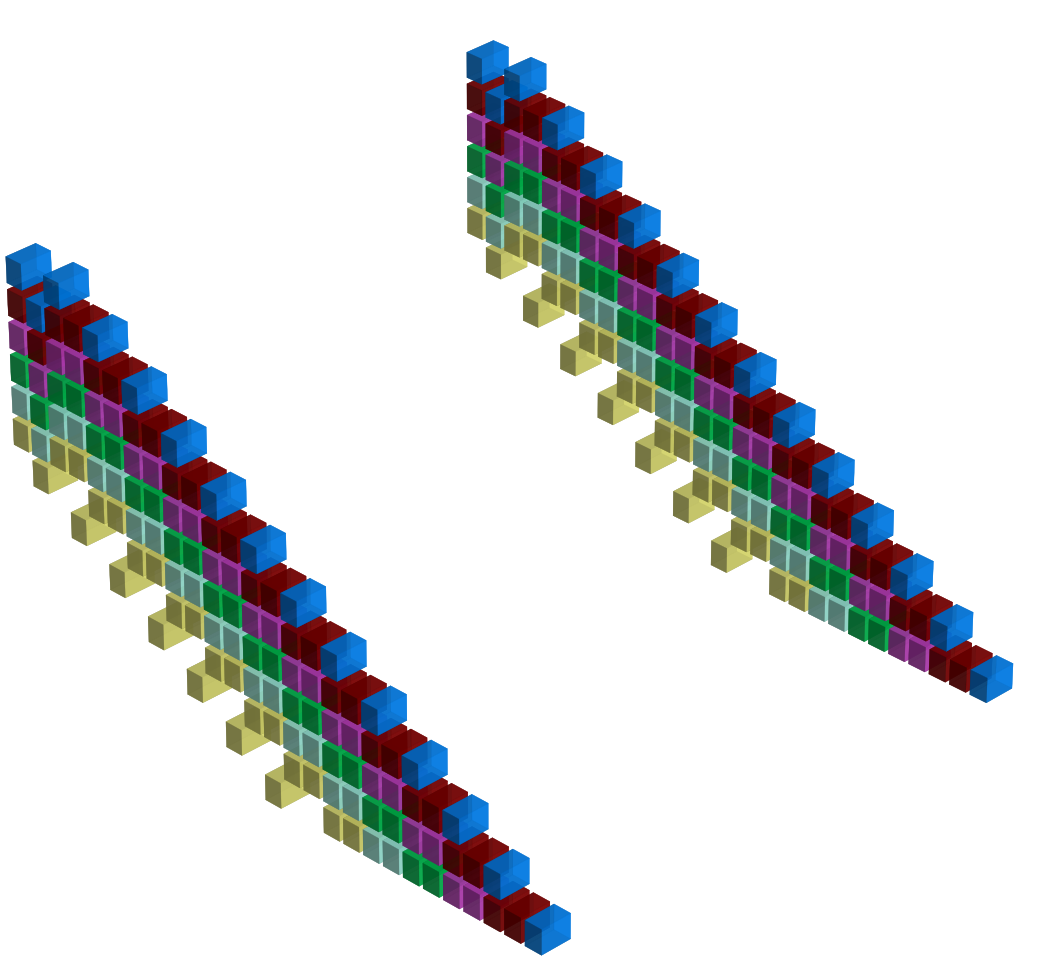
\includegraphics[width=3.2cm]{linemode/symmetries/pattern1-0-45.png}%
    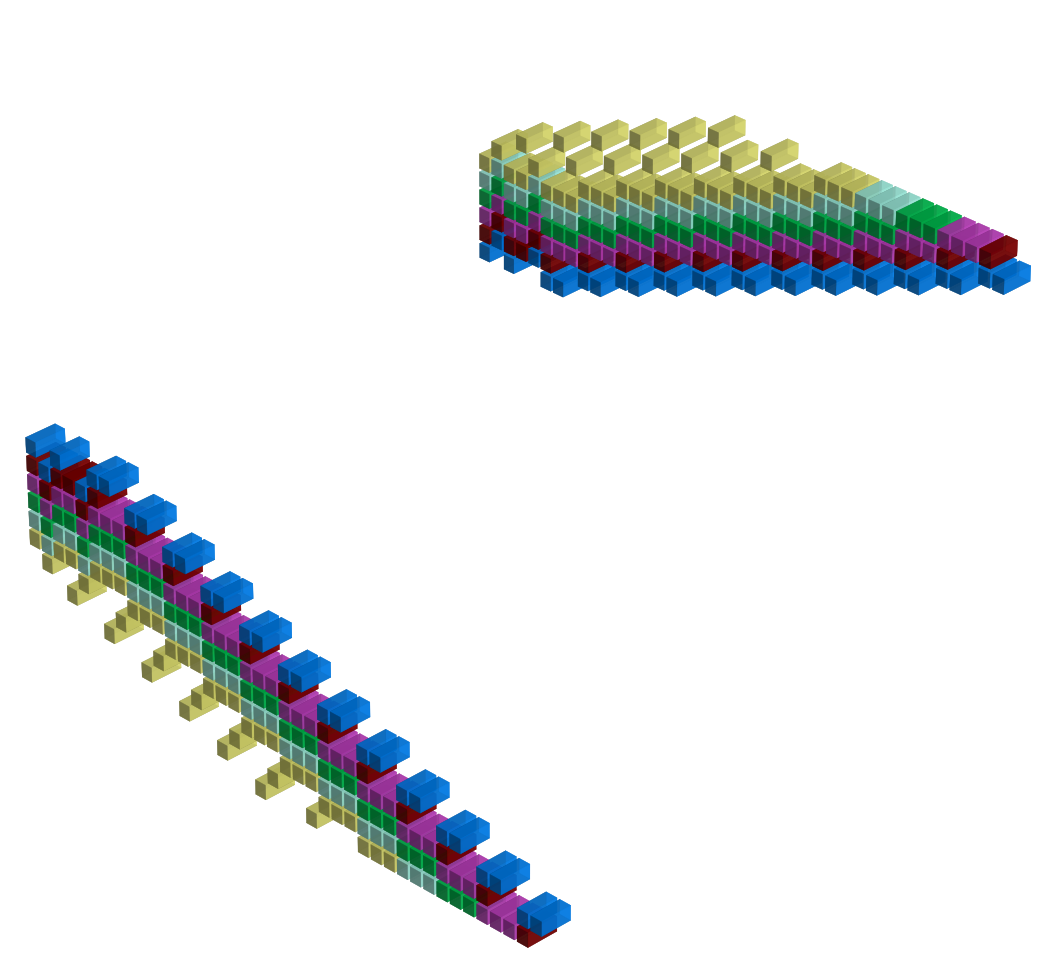
\includegraphics[width=3.2cm]{linemode/symmetries/pattern1-1-45.png}%
    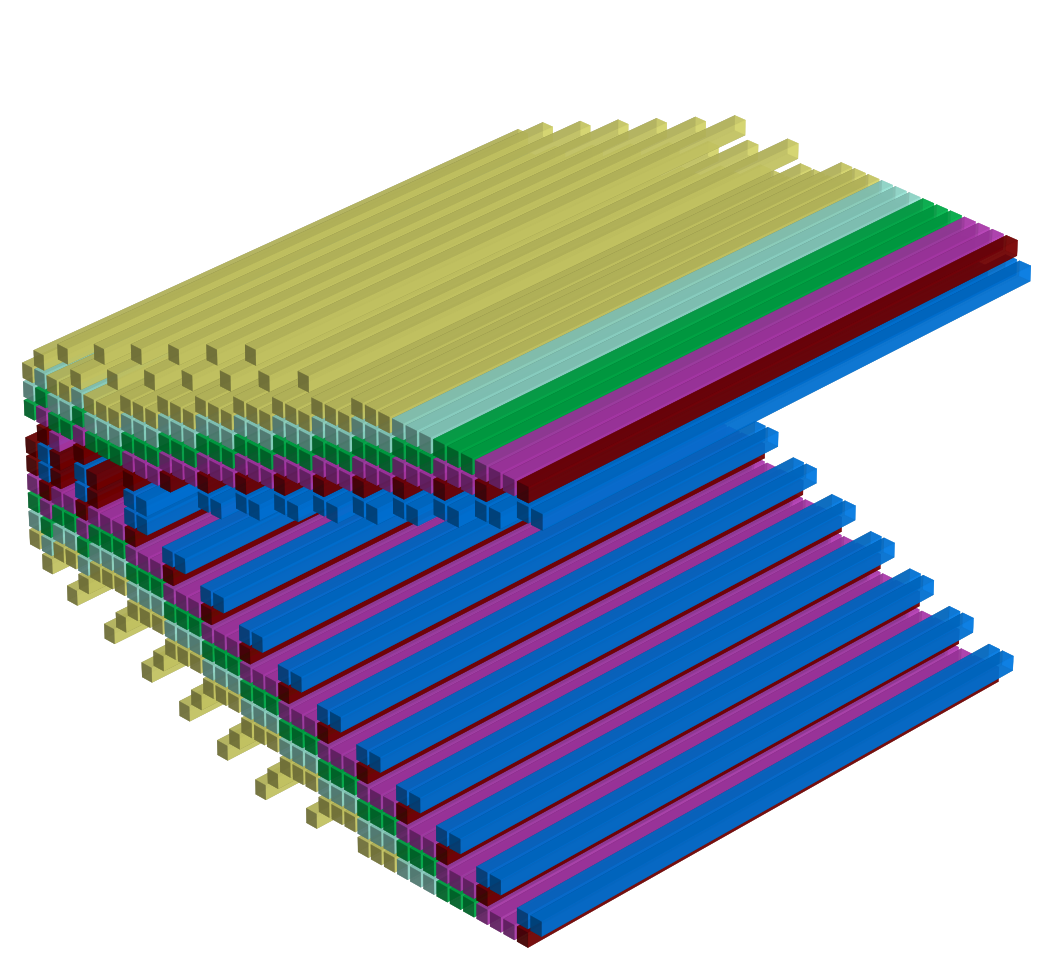
\includegraphics[width=3.2cm]{linemode/symmetries/pattern1-3-45.png}%
    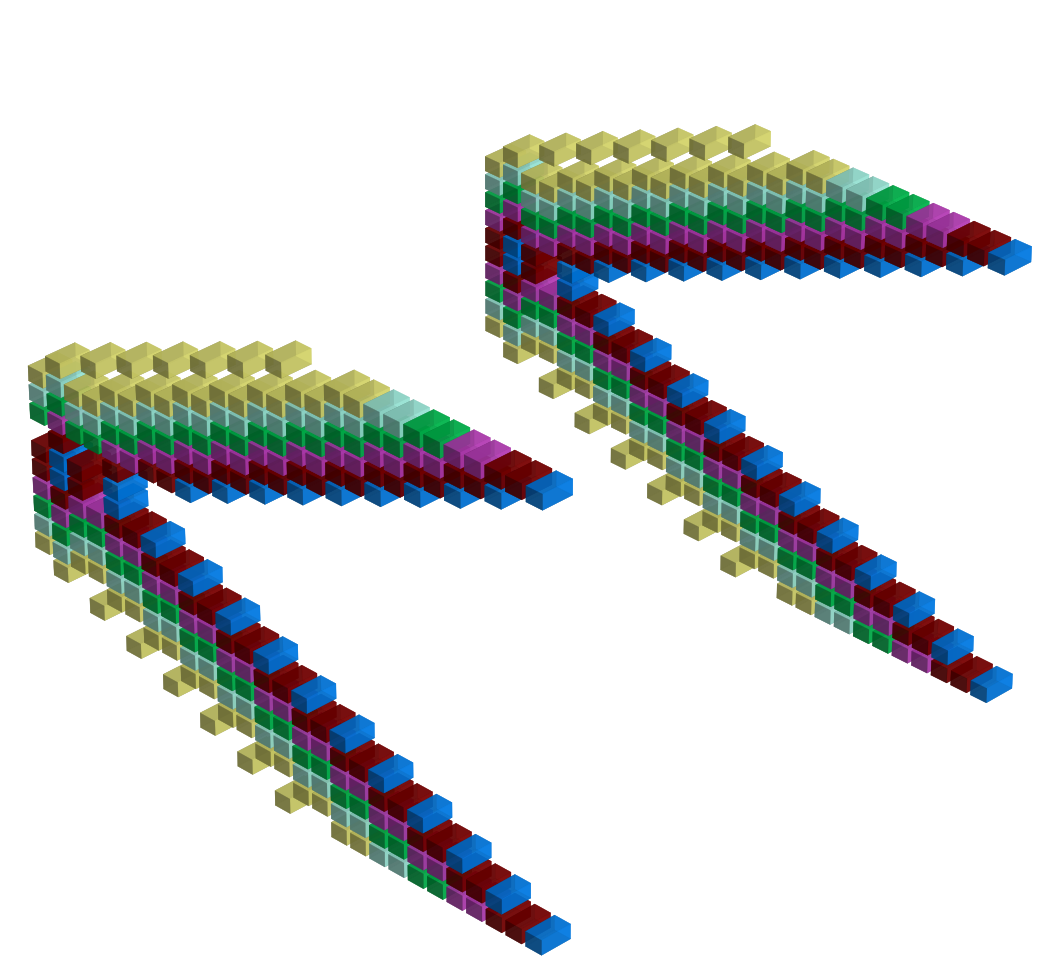
\includegraphics[width=3.2cm]{linemode/symmetries/pattern1-5-45.png}%
    \hspace{0.2cm}
    \caption{
      The different symmetries of Line Mode. 
      }
\end{figure}


\clearpage
